% !TEX root = ../utltcp-paper.tex

We begin by considering in more detail the rationale and requirements for an
unordered and time-lined transport protocol. It is instructive first to
establish TCP as the foundation from which to build, then understand its
negative impact in the context of live and interactive media. Doing so
establishes a set of desirable {\em real-time transport services}.

% We begin by considering in more detail the requirements for the
% transport-layer API that real-time, low-latency applications need. This
% discussion uses the vocabulary established by the Transport Services (TAPS)
% working group at the IETF, allowing us to describe the
% \textit{transport services} our API must provide.
%
% Following this, we discuss the rationale for our use of TCP as the
% foundation for a protocol that provides this API. Finally, we describe the
% high-level design needed to achieve our competing goals of latency
% reduction and wire-compatibility with TCP.

%------------------------------------------------------------------------------
\subsection{TCP Compatible Design Goals}
\label{sec:background-tcp}

Our primary design goal is to improve performance over TCP \emph{for real-time
traffic}, while maintaining the possibility of deployment on the scale of TCP and
UDP. Ossification of the transport layer means this goal can \emph{only} be achieved by
using TCP or UDP as a substrate. This is a limitation that exists in the
Internet because of middleboxes that process packets based on static views of
what is a valid transport. The operation of these middleboxes places two constraints on transport
protocols~\cite{mcquistin:2015:reinterpreting}. First, only packets containing
TCP or UDP are marked as valid by middleboxes; packets containing other transport protocols
are often rejected, and some networks also reject UDP. 
Second, middleboxes may reject valid TCP packets that don't
conform to some limited subset of the TCP protocol that they understand
\cite{honda:2011:extend-tcp}. For example, packets with the
SACK (selective acknowledgement) extension might be rejected by a
middlebox that doesn't understand that extension, and expects only regular
ACK packets.
Reliability and congestion control are desirable features.
These can be implemented by applications running over UDP,
but it is difficult to do this well \cite{RFC5405}. Accordingly,
and because it's more widely accepted by middleboxes, TCP has emerged as
the protocol of choice for real-time multimedia.

% %--------------------------------------------------------------------------
% \subsection{Design Requirements}

% ---------------------------------------------------------------------------
%\subsection{Rationale for TCP Compatibility}

% However, when streams are live and interactive these features are also the
% source of non-network latency. We use an assessment of the underlying mechanisms
% to identify the design requirements.

% Ossification of the transport layer -- due to assumptions made by the numerous
% network middleboxes that believe they understand the transport -means that we
% can only achieve our first goal by using TCP or UDP as a substrate, making
% minimal wire-visible changes. We chose to extend TCP since it provides effective
% congestion control, which is complex to replicate in UDP-based protocols, and
% because UDP is often blocked by enterprise firewalls.

% ------------------------------------------------------------------------------------------------
%\subsection{Design Requirements}
Our secondary goal is to minimize the transport-induced latency on applications.
Given TCP as a necessary substrate, appropriate modifications are needed to meet
our latency goals. TCP introduces latency in part because of (i) the nature of
its congestion control dynamics, and in part by (ii) providing an ordered,
reliable, delivery model using head-of-line blocking and retransmissions. The
former can be addressed using active queue management and/or delay-based
congestion control algorithms, and has been widely studied (e.g., 
\cite{nichols:2012:codel,khademi:2014:new-aqm,brakmo:1994:tcp-vegas}). The
latter issue is more applicable to real-time traffic, and is the subject of our
work.

Figure \ref{diagram:motivation_latency} shows explicitly the impact of
head-of-line blocking. The loss of the third segment causes subsequent segments
to be buffered at the receiver while waiting for the retransmission. Only when
the delayed segment arrives can TCP deliver the in-order sequence to the
application. The impact of retransmitted segments are exacerbated when they push
subsequent segments past the time when they're useful to the
application. Such segments are effectively lost to the application, despite
having been delivered to the host on time. It is these \emph{late losses} that
TCP Hollywood seeks to minimize.

\begin{figure}[t]
 \centering
 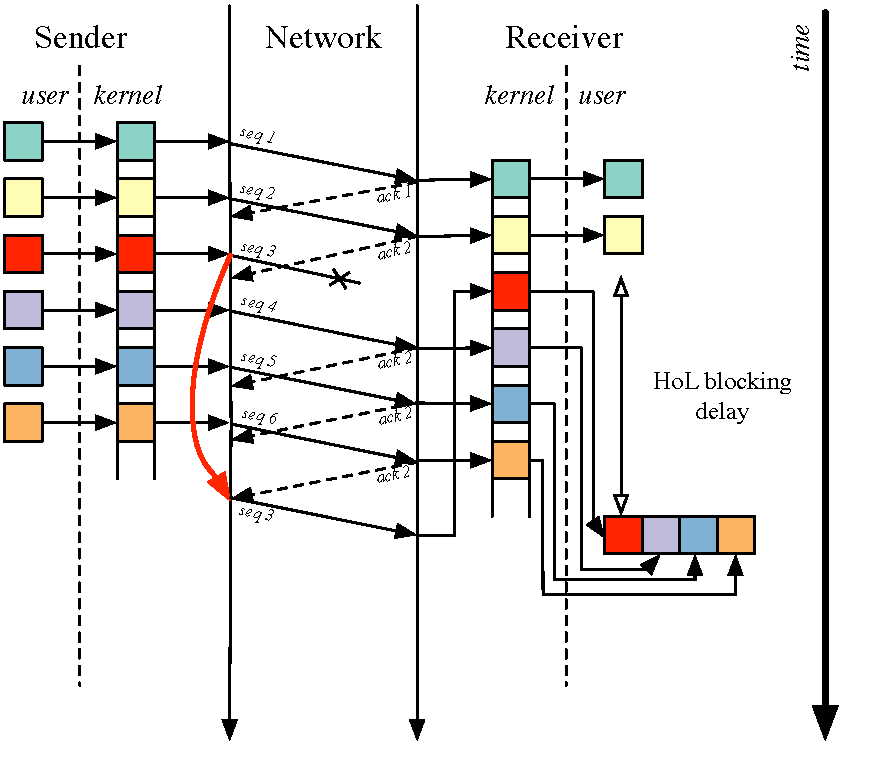
\includegraphics[scale=0.6]{figures/hol-blocking-delay.pdf}
 \caption{The interaction between head-of-line blocking and loss in TCP:
  multiple segments are delayed by a loss, and potentially delivered too late to be useful to the receiver}
\label{diagram:motivation_latency}
\end{figure}

Two requirements follow. First, to eliminate head-of-line blocking,
segments must be delivered as they arrive.  Second, retransmissions should be evaluated
against timing information to ensure delivery of useful data, by allowing
\emph{inconsistent retransmissions} to send new data in a segment that is
retransmitted. So that applications can benefit from out-of-order delivery, a
message-oriented abstraction is needed. Specifically, messages should be
independently useful to the receiver \cite{clark:1990:architecture}. The
following real-time transport services emerge as a result.




%------------------------------------------------------------------------------
\subsection{Service Requirements for Real-time Applications}

In the IETF, the Transport Services (TAPS) working group provides a vocabulary
for discussing transport protocol components~\cite{taps}. We use their
vocabulary to describe the transport services we believe are needed for
real-time multimedia. Details, as well as an abstract API, may be
found in~\cite{McQuistinANRW:2016}.

\textbf{Timing} is an implicit and salient attribute of real-time media
applications. Timing requirements determine {\em deadlines} to present media to
the application, i.e., to play audio and render video. Deadlines depend on the
nature of the application. Interactive application deadlines, such as for
telephony, video conferencing, or telepresence, range from tens to hundreds of
milliseconds. Non-interactive broadcast or on-demand streaming applications can
tolerate deadlines on the order of seconds.

Networked multimedia timing and deadline services are unusual among real-time systems. Consider that data that misses its deadline arrives too late to be usefully rendered to the user; yet that same data may be used by the application to complete a predictive decoding chain. This suggests a need to redefine the nature of reliability and ordering.

% \textbf{Timing} is a fundamental characteristic of low-latency application
% traffic, and it is foundational for our API: the other services follow from
% it. The data generated by these applications has a relative deadline
% associated with it -- the duration in which the data can be considered to
% be useful to the receiver. These relative deadlines are dependent on the
% latency requirements of the application; interactive applications (e.g.,
% telephony, video conferencing) have hard latency bounds, while
% non-interactive applications have softer bounds.

\textbf{Partial Reliability} services acknowledge that a transport might be unable to
deliver data by a given deadline. A retransmission that fails its timing
requirements leads to play-out stalls. This causes applications to block, and is
a primary cause of poor user experience. Accordingly a transport protocol
designed to meet deadlines should support partial reliability, and retransmit
only data is useful to the application.

% Supporting the timing service over a lossy, best-effort network requires
% support for \textbf{partial reliability}. There is some probability that
% packet loss will occur, and that the lost packets will have to be
% retransmitted. Since retransmissions themselves may be lost, the delay
% introduced by a fully reliable transport service is unbounded: this is
% incompatible with the timing service. Data should only be transmitted if it
% is likely to useful on reception.

\textbf{Message-oriented Dependency} services culminate from timing and partial
reliability services. Data should be transmitted to the receiver only when the
receiver can play the data in time, or when the data is needed as part of the
decoding chain. This service is further complicated because the sender should
never transmit data that relies on previous transmissions that were never
received. Managing dependencies in this fashion requires application-layer
framing~\cite{clark:1990:architecture} to provide a {\em message-oriented}
service that maintains, and transmits along, application data unit (ADU)
boundaries.

Message orientation also provides a foundation for {\em multi- or sub-stream services}. Media content can be composed of multiple streams of data, each with its own data characteristics. Audio and video, for example, may be separated into streams with different priorities, message sizes, and bitrates. Message-orientation may also be exploited in multipath environments. An independent {\em multipath service}, for example, may increase utility by scheduling packet transmissions by matching sub-path properties with sub-stream characteristics.

% A \textbf{dependency management} service is required as a result of partial
% reliability: data might depend on earlier data that was not received
% successfully, rendering it useless to the receiver. Exposing dependency
% information to the transport layer prevents such data from being sent.
%
% A partial reliability service also requires a \textbf{messaging} service to
% maximise the utility of each data packet. The application should transact
% in application data units: discrete blocks of data that are independently
% useful to the receiving application. To minimise latency, these messages
% should be delivered to the application in the order that they arrive.
%
% A \textbf{multistreaming} service is desirable. Some target
% applications comprise multiple streams (for example, distinct audio
% and video streams in a typical multimedia application). Each of these
% streams has different characteristics (e.g., message sizes, sending rates)
% that should be exposed to the transport layer.

% With metadata about different streams, a \textbf{multipath} service is
% needed to map these to different paths within the network. This mapping
% should match the characteristics of each stream with the properties of each
% network path, increase the utility of the network.

\textbf{Connections and Congestion Control} are critically important.
Networked multimedia content is increasingly encoded at variable or
adaptive bitrates, or both. Applications, user experience, and network
utilization, would be best served by the ability to respond to changes in
available bandwidth. We argue that real-time transport should rely upon,
but be agnostic to, TCP congestion control to ensure co-existence on the
wider Internet. TCP Hollywood uses TCP congestion control unchanged, and
can make immediate use of advances in TCP congestion control as they
become available.

An explicit connection-oriented service may be a lesser requirement, given
per-flow state at the endpoints is sufficient to provide 
congestion control. However, signalling messages indicating
start and end of connections can, for example, ease NAT traversal and
facilitate firewall management. Accordingly, the availability of a
connection-oriented service is desirable.

%
%  is required to protect the network, and the
% other applications that use it. The congestion control algorithm should
% account for the latency-sensitive nature of the applications. 
% Congestion control algorithms would benefit from a \textbf{connections}
% service, making use of per-connection metadata. Beyond this, having
% explicit connection setup and teardown signals may benefit in-network
% services, such as NAT traversals and firewall pinholing.
%
%
% % In the next section we present the TCP Hollywood architecture, alongside the design
% % elements that preserve TCP semantics and ensure wire-line compatibility.


% With both a message-oriented
% abstraction and timing information, the collection of message dependency
% information follows. This increases the application-awareness of the
% transport layer.
